\setstretch{1.0}
\chapter{5-Dimensional dynamic connectivity}\label{chapter_cca}

Increasing evidence suggests that functional connectivity is non-stationary in time. Further, electrophysiological measurements show that connectivity is dependent on the frequency band of neural oscillations. It is also conceivable that networks exhibit a degree of spatial non-stationarity, i.e. the large scale networks that we observe may result from the time average of multiple transiently synchronised sub-networks, each with their own spatial signature. This means that the next generation of neuroimaging tools to compute functional connectivity must account for spatial, spectral and temporal non-stationarity. Here, we present a means to achieve this 5-dimensional picture via application of windowed canonical correlation analysis (CCA) to source space projected MEG data. We describe generation of time-frequency connectivity plots, showing the temporal and spectral distribution of coupling between brain regions. Moreover, CCA applied across voxels provides a means to assess spatial non-uniformity within short time-frequency windows. The feasibility of this technique is demonstrated in simulation and in a resting state MEG experiment in a single subject where we elucidate multiple distinct 5-dimensional modes of covariation between the left and right sensorimotor areas.

\doublespacing
\section*{Introduction}
So far in this thesis we have discussed multiple technical challenges associated with measuring functional connectivity using non-invasive electrophysiological data. We have discussed methods to reconstruct data in source space, allowing us to infer the spatial origin of neural signals. We then highlighted that these reconstruction methods, due to the ill-posed nature of the problem they are trying to solve, introduce signal leakage which if not properly controlled will artefactually inflate the magnitude of functional connectivity. Having discussed methods to reduce leakage, we then showed that there are many different ways to assess functional connectivity, each with their unique strengths and weaknesses. With the decision to focus on the Amplitude Envelope Correlation (AEC) method we now focus on applying what has be learnt to experimental data. In particular, we expand the methods of univariate AEC analysis, into a multivariate framework. The reason for this, as discussed in Chapter \ref{chap_intro}, is that if functional connections are dynamic in time, then it is with strong possibility that these connections are also non-stationary in space. Methods which can capture this non-stationarity across time and space (and even frequency, which has been shown to have a profound effect on electrophysiological functional connectivity \citep{Brookes2012a}) will likely reveal dynamic properties of functional connections previously unseen in neuroimaging. In what follows, Section \ref{sec_cca_theory} introduces the theory of canonical correlation analysis (CCA), a multivariate extension of Pearson correlation -- along with methodology to extend signal orthogonalisation (necessary for the removal of signal leakage) between multivariate datasets. Section \ref{sec_cca_sims} presents a series of simulations to show that multivariate leakage correction rejects the null hypothesis and demonstrates the ability of CCA to find correlations between large volumes of brain. In Section \ref{sec_cca_real} we then apply these methods on real MEG resting state data in a single subject and show how functional connectivity in the sensorimotor network fluctuates in time and frequency. Furthermore, we reveal reveal unique spatial modes of sensorimotor connectivity can be revealed in a single subject..

\section{Theory}\label{sec_cca_theory}
\subsection{Source Localisation and Selection of Voxels Clusters}
Characterisation of functional connectivity between two voxel clusters using MEG data necessarily requires that electrophysiological signals are assessed in source space (i.e. extra-cranial magnetic field data are projected into the brain). As discussed in Chapter \ref{chapter_meg_source}, there are several advantages of source space projection in connectivity assessment \citep{Scoffelen2009}. Firstly results can be overlaid directly onto structural brain images, enabling direct interpretation with respect to underlying anatomy. Secondly, source localisation (via adaptive techniques such as beamforming) reduces artefacts from MEG data \citep{Sekihara2001,Sekihara2006}, meaning that the signal to noise ratio (SNR) of source space projected data is generally higher than the SNR of raw data in channel space. This second point is often overlooked, but is of critical importance in this context since artefacts caused by common interference across MEG channels (from e.g. the heart) may generate spurious correlation \citep{Brookes2011a}. Here, source space projection is achieved via beamforming \citep{VanVeen1997,Robinson1999,Sekihara2001,Brookes2008} for reasons established in Chapter \ref{chapter_meg_source}.

In what follows, our aim is to measure connectivity via assessment of the interaction between projected signals within two spatially separate voxel clusters. We shall refer to these as the ‘seed’ cluster and the ‘test’ cluster. Voxels were defined at the vertices of a regular (8 mm) grid spanning these regions. A single current orientation was estimated for each voxel, based on a non-linear search for the orientation of maximum signal to noise ratio; this search was limited to the tangential plane due to the relative insensitivity of MEG to radially oriented currents \citep{Robinson1999}. For simplicity the theoretical description pertains to a single frequency band; although multiple bands are easily incorporated in the same framework by frequency filtering and sequential application.

Following beamformer projection of MEG data, the electrical source timecourses for all voxels within the seed and test volumes are henceforth represented by the projected data matrices \textbf{X} and \textbf{Y}. \textbf{X} represents data from the seed cluster and has dimensions $f\Delta\times N_s$, where $\Delta$ is the duration of the experiment (in seconds), \textit{f} is the MEG sampling rate (in Hz) and $N_s$ is the number of voxels contained within the seed cluster. \textbf{Y} represents data from the test location and is of dimension  $f\Delta\times N_t$, where $N_t$ is the number of voxels contained within the test cluster. All subsequent operations are performed on these two matrices.

\subsection{Multivariate Correction for Signal Leakage}\label{sec_multivar_leak}
Methods to reduce leakage - either by regession of signals or modifying functional connectivity metrics (as discussed in Chpater \ref{chapter_fc_and_leakage}) typically focus on leakage between two voxels. Here however, we aim to probe connectivity between larger cortical volumes (clusters). Increasing the size of the brain volumes studied makes the chances of observing signal leakage statistically more likely, and for this reason an effective means to eliminate leakage between the data matrices \textbf{X} and \textbf{Y} is of key importance. It is well known that leakage gives rise to a zero-phase-lag linear interaction between projected signals, this fact has been exploited in previous methods \citep{Nolte2004,Stam2007,Brookes2012b,Hipp2012} where zero-phase-lag interaction is removed prior to connectivity assessment. In this chapter we implement a multivariate extension to this previous work \citep{Brookes2012b,Hipp2012} in which linear regression is employed to remove any zero-phase-lag interaction between the seed and test regions. 

To efficiently remove a linear projection of \textbf{X} on \textbf{Y}, we first reformulate each matrix into an orthogonal basis set; a condition that is never met in MEG since the columns of \textbf{X} and \textbf{Y} comprise timecourses from neighbouring voxels which will always contain similar signals due to the inherent smoothness of beamformer reconstruction (and would lead to inflated degrees of freedom in the subsequent multivariate test). To orthogonalise the columns of \textbf{X} and  \textbf{Y}, we employ a technique based on eigenvalue decomposition. We first compute the covariance matrices of \textbf{X} and \textbf{Y} thus:

\begin{align}
\mathbf{C}_{XX} &= \mathbf{X}^T\mathbf{X} \\
\mathbf{C}_{YY} &= \mathbf{Y}^T\mathbf{Y}.
\end{align} These covariance matrices are reduced to their constituent eigenvectors and eigenvalues thus:

\begin{align}
\mathbf{C}_{XX} &= \mathbf{U}_X\mathbf{S}_X\mathbf{U}_X^T \\
\mathbf{C}_{YY} &= \mathbf{U}_Y\mathbf{S}_Y\mathbf{U}_Y^T.
\end{align} The columns of $\mathbf{U}_X$ and $\mathbf{U}_Y$ represent the eigenvectors of $\mathbf{C}_{XX}$ and $\mathbf{C}_{YY}$ respectively. $\mathbf{S}_X$ and  $\mathbf{S}_Y$ are diagonal matrices whose elements correspond to the eigenvalues of $\mathbf{C}_{XX}$ and $\mathbf{C}_{YY}$. Having found the eigenvectors, it is possible to construct new, orthogonalised versions of \textbf{X} and \textbf{Y} which we term $\mathbf{X}_o$ and  $\mathbf{Y}_o$:

\begin{align}
\mathbf{X}_o &= \mathbf{X}\mathbf{U}_X\\
\mathbf{Y}_o &= \mathbf{Y}\mathbf{U}_Y.
\end{align} In principle at this stage we could also choose to reduce the dimensionality of the problem (by keeping fewer columns in $\mathbf{U}_X$ and $\mathbf{U}_Y$), but we keep all orthogonal components, since we have a large number of temporal degrees of freedom at our disposal.  Having collapsed \textbf{X} and \textbf{Y} into a set of mutually orthogonal vectors (i.e. a basis set) we can now remove the leakage (defined as a linear correlation of $\mathbf{X}_o$ and $\mathbf{Y}_o$) between the two voxel clusters using a multivariate general linear model, where $\mathbf{Y}_o$ is expressed as a linear combination of the features contained in $\mathbf{X}_o$:

\begin{equation}\label{eqn_4_07}
\mathbf{Y}_o = \mathbf{X}_o\mathbf{\beta}_L+\mathbf{Y}_{oc}.
\end{equation} Here, $\mathbf{\beta}_L$ represents the combination of orthogonalised features that best describes linear leakage and can be found using

\begin{equation}
\mathbf{\beta}_L = \mathbf{X}_o^+\mathbf{Y}_o,
\end{equation} where $\mathbf{X}_o^+$ denotes the Moore-Penrose pseudoinverse of $\mathbf{X}_o$. Notice that the ‘error’ term, $\mathbf{Y}_{oc}$, in Equation \ref{eqn_4_07} actually represents the corrected data matrix for the test cluster and, following computation of $\mathbf{\beta}_L$, can be calculated as  $\mathbf{Y}_{oc} = \mathbf{Y}_{o} - \mathbf{X}_o\mathbf{\beta}_L$. Finally, the corrected signal $\mathbf{Y}_{oc}$ can be transformed from the orthogonalised signal subspace back to voxel space using the equation:

\begin{equation}
\mathbf{Y}_c = \mathbf{Y}_{oc}\mathbf{U}_Y^T.
\end{equation} Leakage correction in this way means that there is no linear zero-phase-lag interaction between any linear combination of the columns in \textbf{X} and $\mathbf{Y}_c$ . However as in the single voxel approach (Chapter \ref{chapter_fc_and_leakage}; \citealp{Brookes2012b,Hipp2012}), it should be noted that this comes at the expense of any genuine zero-phase-lag interactions which have been demostrated to exist in invasive recordings \citep{Singer1999,Leopold2003}.

\subsection{Non-Stationarity and Canonical Correlation Analysis}
Having corrected for leakage between voxel clusters we now aim to probe the existence of a statistical interdependency between the voxel timecourses from the seed cluster \textbf{X}, and the corrected test cluster $\mathbf{Y}_c$. Since we aim to assess temporal correlation between band limited amplitude envelopes, the individual columns of \textbf{X} and $\mathbf{Y}_c$ (i.e. the voxel timecourses) are Hilbert transformed to obtain the analytic signal (as described in Section \ref{sec_3_hilbert}); the absolute value of this analytic signal is then computed yielding two new matrices, $\mathbf{E}_X$ (dimension $f\Delta\times N_s$) and $\mathbf{E}_Y$ (dimension $f\Delta\times N_s$) whose columns comprise the band limited amplitude envelope signals in different voxels.

$\mathbf{E}_X$ and $\mathbf{E}_Y$ are representative of the whole experiment, (i.e. they each contain $f\Delta$ rows), however the methodology needs to account for non-stationarity in time. For this reason, we now introduce a sliding window of temporal width $\delta$ (in seconds) which is allowed to move in time, and we only assess temporal correlation between clusters within these windows. This concept is shown graphically in Figure \ref{fig_4_1}, where the red dotted lines represent the window boundaries. The windowed seed cluster envelope matrix is denoted as $\mathbf{W}_X$  (which has dimension $f\delta\times N_s$) and the windowed test cluster envelope matrix as $\mathbf{W}_Y$ (which has dimension $f\delta\times N_t$). Having selected a window, we test for a relationship between the seed and test clusters using a multivariate general linear model, in exactly the same way as described above (Equation \ref{eqn_4_07}). Here however, note that we are testing for a linear relationship between the amplitude envelopes of the signal, and not for a linear zero-time-lag relationship between the raw signals. 

As with leakage correction, we first account for the fact that separate columns of $\mathbf{W}_X$ or $\mathbf{W}_Y$ are likely to be correlated; again recall that these columns represent envelope timecourses from reconstructed voxels in close spatial proximity. In order to remove this redundancy, and to constrain the degrees of freedom of our test (which will impact on the length of the time window) we decompose these data in a fixed number (\textit{d}) of orthogonal spatial modes.  There are multiple methodologies to impose orthogonality and here eigenvalue decomposition was employed. The covariance matrices for $\mathbf{W}_X$ and $\mathbf{W}_Y$ were computed as:

\begin{align}
\mathbf{W}_{X}^T\mathbf{W}_{X} &= \mathbf{V}_X\mathbf{T}_X\mathbf{V}_X^T \\
\mathbf{W}_{Y}^T\mathbf{W}_{Y} &= \mathbf{V}_Y\mathbf{T}_Y\mathbf{V}_Y^T.
\end{align} The columns of $\mathbf{V}_X$ and $\mathbf{V}_Y$, which represent the eigenvectors of the covariance of $\mathbf{W}_X$ and $\mathbf{W}_Y$ respectively, were then truncated, leaving only \textit{d} eigenmodes. Following this, two new matrices are constructed such that:

\begin{align}
\mathbf{W}_{Xo} &= \mathbf{W}_X\mathbf{V}_{XT} \\
\mathbf{W}_{Yo} &= \mathbf{W}_Y\mathbf{V}_{YT}.
\end{align} Where $\mathbf{W}_{Xo}$ and $\mathbf{W}_{Xo}$ have \textit{d} columns and $f\delta$ rows. It is important to note here that at least $4d$ independent temporal observations are required for the multivariate test to be reliable; and this sets the trade-off between the number of spatial features examined and window length ($\delta$). The orthogonal nature of the columns in $\mathbf{W}_{Xo}$ and $\mathbf{W}_{Yo}$ facilitates unambiguous application of the multivariate GLM such that:

\begin{equation}
\mathbf{W}_{Yo} = \mathbf{W}_{Xo}\mathbf{\beta}+\mathbf{\epsilon}
\end{equation} Where $\mathbf{\beta}$ is the matrix of regression coefficients best predicting $\mathbf{W}_{Yo}$ from $\mathbf{W}_{Xo}$. This whole procedure is depicted graphically in Figure \ref{fig_4_1}, where the number of features maintained following truncation of the eigenvectors (\textit{d}) is 5. 

\begin{figure}[h!]
	\begin{center}
		\includegraphics[width=0.89\linewidth]{./images/chapter4/figure_1.png}\caption{Schematic diagram of the windowed multivariate GLM to test for temporal correlation between band limited amplitude envelopes. The time window, represented by the red dashed lines,  allowing us to measure  functional connectivity as a function of time.}\label{fig_4_1}
	\end{center}	
\end{figure}

\clearpage
Following computation of $\mathbf{\beta}$, it is possible to apply previously established CCA methods \citep{Soto2009,Soto2010,Barnes2011,Brookes2012b}. We first compute the covariance explained by the estimate $\mathbf{W}_{Xo}\mathbf{\beta}$ as:

\begin{equation}
\mathbf{H} = ( \mathbf{W}_{Xo}\mathbf{\beta})^T( \mathbf{W}_{Xo}\mathbf{\beta}).
\end{equation} In addition, one can compute the unexplained covariance as: 

\begin{equation}
\mathbf{R} = (\mathbf{W}_{Yo} - \mathbf{W}_{Xo}\mathbf{\beta})^T(\mathbf{W}_{Yo} - \mathbf{W}_{Xo}\mathbf{\beta}).
\end{equation} It then becomes possible to compute the matrix

\begin{eqnarray}
\mathbf{D} =  \mathbf{R}^{-1}\mathbf{H},
\end{eqnarray} which corresponds to the ratio of the explained covariance to unexplained covariance. In a univariate sense, this is equivalent to an F-statistic. In the multivariate case, the eigenvalues, $\mathbf{S}_D$ , and the associated eigenvectors, \textbf{A}, of \textbf{D} are defined thus:

\begin{equation}
\mathbf{D} = \mathbf{AS}_D\mathbf{A}^T.
\end{equation} The individual columns of \textbf{A} (i.e. the eigenvectors) are known as the canonical vectors in $\mathbf{W}_{Xo}$ and show explicitly how to combine the individual orthogonal columns of $\mathbf{W}_{Xo}$ to best explain the variance observed within and across the columns of $\mathbf{W}_{Yo}$. In a similar way the canonical vectors in $\mathbf{W}_{Yo}$ can be computed as:


\begin{equation}
\mathbf{B} = \mathbf{\beta A}
\end{equation} The canonical vectors \textbf{A} and \textbf{B} can be used to calculate the canonical variates; these comprise the composite timecourses; that is to say the weighted sum of the columns of $\mathbf{W}_{Xo}$ and $\mathbf{W}_{Yo}$ that maximise temporal correlation, in the window of interest, between the seed and test clusters. The canonical variates are given by
\begin{equation}
\begin{aligned}
\mathbf{K}_{Xo} &= \mathbf{W}_{Xo}\mathbf{B} \\
\mathbf{K}_{Yo} &= \mathbf{W}_{Yo}\mathbf{A}
\end{aligned}
\end{equation}
It then becomes possible to compute the canonical correlation coefficients as

\begin{equation}
\mathbf{r}_\text{can} = \frac{\mathbf{K}_{Xo}^T\mathbf{K}_{Yo}}{\sqrt{\mathbf{K}_{Xo}^T\mathbf{K}_{Xo}\mathbf{K}_{Yo}^T\mathbf{K}_{Yo}}}
\end{equation} (Note that the square root represents an element by element square root.) The matrix $\mathbf{r}_\text{can}$ has dimension $d\times d$ and the elements represent correlation coefficients between the various eigenmodes of correlation. As the eigenmodes are by definition orthogonal, all off-diagonal elements in this matrix are zero and the diagonal elements represent a single canonical correlation coefficient per eigenmode. For the majority of this chapter we focus on the first eigenmode (in which most of the variance is explained), but there is no reason why other modes could not be examined. 

Finally, the canonical vectors can be projected back onto the individual voxels within the seed and test locations. This generates images showing the optimal weighted sum of voxels in the seed cluster that maximally correlate with the optimal weighted sum of voxels in the test cluster. The voxel weightings in the seed location are given by:

\begin{equation}
\mathbf{I}_{WX} = \mathbf{BV}_X^T.
\end{equation} Likewise, the voxel weightings in the test cluster are given by:

\begin{equation}
\mathbf{I}_{WY} = \mathbf{AV}_Y^T.
\end{equation} The above theoretical treatment of beamformer projected MEG data allows for the computation of the canonical correlation coefficient within each time window, along with images, $\mathbf{I}_{WX}$ and $\mathbf{I}_{WY}$, which describe the combination of voxels which maximise that correlation. Letting the window shift in time facilitates assessment of temporal and spatial structure in correlation. Finally, sequential application to multiple frequency bands enables measurement of the spectral signature of correlation. 
 
\subsection{Statistical testing via phase randomisation}\label{phase_randomisation}
Application of windowed CCA requires careful statistical testing since spurious changes in the temporal profile of correlation can be generated simply as a result of changes in the Fourier components contained within the envelope signals. For example, consider two separate time windows, A and B; in time window A the windowed envelope signals $\mathbf{W}_{X}$ and $\mathbf{W}_{Y}$ contain correlated Gaussian noise (i.e. exhibit an even distribution across all Fourier components), whereas in time window B those envelope data become coloured (i.e. dominated by a small number of Fourier components). In such a case, the number of temporal degrees of freedom in the data is reduced, and the value of the canonical correlation coefficients $\mathbf{r}_\text{can}$ will necessarily increase. This increase is due entirely to the change in spectral structure of the signals and does not represent a genuine change in functional connectivity between the two clusters. Put another way, the background temporal structure in the envelope data will yield non-zero source space correlations that will fluctuate significantly, even if all parameters relating to functional connectivity itself are stationary. For this reason, a robust and reliable statistical technique to account for these ‘trivial’ changes in functional connectivity must be employed. 

The technique used here involves generating surrogate envelope data based upon a phase randomisation process \citep{Prichard1994}. For univariate data, phase randomisation is a simple procedure in which, given a univariate time series, $w(t)$, we first compute its discrete Fourier transform $F\big[w(t)\big]=A(f)e^{i\phi(f)}$ where $F$ denotes a Fourier transform, $A(f)$ is the amplitude of each Fourier component and $\phi(f)$ is the phase. A phase randomised signal, $\tilde{w}(t)$ can then be generated by rotation of the phase of each Fourier component by a random angle, $\xi(f)$, which is chosen uniformly in the range $0 < \xi < 2\pi$ (note that $\xi(f)$ differs for each rotated Fourier component). Mathematically the phase randomised signal is then given as 

\begin{equation}
\tilde{w}(t) = F^{-1}\Big[A(f)e^{i(\phi(f)+\xi(f))}\Big]. \label{eqn_4_23}
\end{equation} Note that $\tilde{w}(t)$ has the desirable property that the magnitude of all of the Fourier components (i.e. the power spectrum) is the same as for the original data, and by the Wiener-Khintchine theorem \citep{Prichard1994} so is the autocorrelation function. Equation \ref{eqn_4_23} describes a univariate case, however $\mathbf{W}_{X}$ and $\mathbf{W}_{Y}$ are multivariate measurements. In the multivariate case, we not only wish to preserve the Fourier properties of a timeseries, but also the linear correlations between the columns of both $\mathbf{W}_{X}$ and $\mathbf{W}_{Y}$; mathematically, we wish to preserve the structure of the covariance matrices $\mathbf{W}_{X}^T\mathbf{W}_{X}$ and $\mathbf{W}_{X}^T\mathbf{W}_{X}$. This can also be achieved via phase randomisation, if the same random sequence $\xi(f)$ is added to each Fourier transformed timecourse (i.e. each Fourier transformed column of $\mathbf{W}_{X}$ and $\mathbf{W}_{Y}$). Mathematically:

\begin{equation}
\tilde{w}_j(t) = F^{-1}\Big[F\big[w_j(t)\big]e^{i\xi(f)}\Big]. \label{eqn_4_24}
\end{equation} where $w_j(t)$ represents the j\textsuperscript{th} column of $\mathbf{W}_{X}$ and $\mathbf{W}_{Y}$; $\tilde{w}_j(t)$ represents the equivalent j\textsuperscript{th} column of a surrogate matrix, which we term $\tilde{\mathbf{W}}_{X}$ or $\tilde{\mathbf{W}}_{Y}$. Note that, when constructed in this way, $\tilde{\mathbf{W}}_{X}$ and $\tilde{\mathbf{W}}_{Y}$ each individually contain the same power spectra and cross correlation structure as $\mathbf{W}_{X}$ and $\mathbf{W}_{Y}$ respectively. However, the phase randomisation means that there should be no correlation between $\tilde{\mathbf{W}}_{X}$ or $\tilde{\mathbf{W}}_{Y}$. This being the case, iterative construction of successive realisations of  $\tilde{\mathbf{W}}_{X}$ and $\tilde{\mathbf{W}}_{Y}$ allow for the generation of a null distribution, independently for each time window considered by the windowed CCA. This, in turn, allows for the generation of a dynamic statistical threshold, formed independently for each time window which accounts for trivial correlations caused by changes in the Fourier components of the envelope signals.

\section{Simulations}\label{sec_cca_sims}
The theoretical analyses described above were applied to a set of simulations in order to test the applicability of the technique. All simulations were based on the geometry and data collection parameters of the third order synthetic gradiometer configuration of a 275 channel CTF whole head MEG system (MISL, Coquitlam, Canada) with 5cm baseline axial gradiometers. The brain anatomy and head location were based on a real experimental recording session and the simulated sampling rate was 600Hz. In all cases a multiple local sphere volume conductor head model \citep{Huang1999} was employed and the forward solution was based on the dipole model derived by \cite{Sarvas1987}.

\subsection{Null simulation and leakage correction}
\subsubsection{Methodology} \label{subaec_sim_method}
The purpose of our primary simulation was to assess the performance of CCA, with and without multivariate leakage correction as described in Section \ref{sec_multivar_leak}. In order to test the effectiveness of leakage correction, null data were simulated. Six spatially separate sources were generated with dipoles located approximately along the motor strip; these locations are shown in Figure \ref{fig_4_2}. For all six dipoles, the dipolar orientation was tangential to the global sphere radius (computed relative to the mean of all of the local spheres) but randomised with respect to the azimuthal direction. The source timecourses were generated as phase randomised versions of genuine (MEG measured) electrophysiological signals (490s in duration), which were estimated from the motor cortex of a single individual during a resting state experiment. Univariate phase randomisation, as described by Equation \ref{eqn_4_23}, was applied in order to maintain the approximate $1/f$ power spectral distribution of the neural oscillatory signal, whilst destroying any genuine correlation that might exist between the neural signals used. In this way, no interaction was expected between any of the six simulated sources, meaning that if significant interactions were observed they were entirely spurious and likely due to signal leakage. Signals were frequency filtered to the beta band and all sources were given amplitude of 3 nAm. Note that beta oscillations were used since previous work has shown that the strongest interactions between the left and right sensorimotor areas occur in this frequency band \citep{Brookes2011a}. The simulated dipole timecourses were projected through forward solutions for each dipole location/orientation and summed, yielding a simulated sensor space signal matrix. Additive noise data were generated by experimental recording. A 490 s MEG recording was made using the third order synthetic gradiometer configuration of a 275 channel CTF MEG system at a sampling rate of 600 Hz, with no subject in the scanner. These ‘empty room’ data formed the noise matrix which was added to the signal matrix thus generating a simulated MEG data set. The signal to noise ratio, defined as the ratio of the Frobenius norm of the signal matrix to the Frobenius norm of the noise matrix, was calculated as 1.6 (mean across runs). 

\begin{figure}[h]
	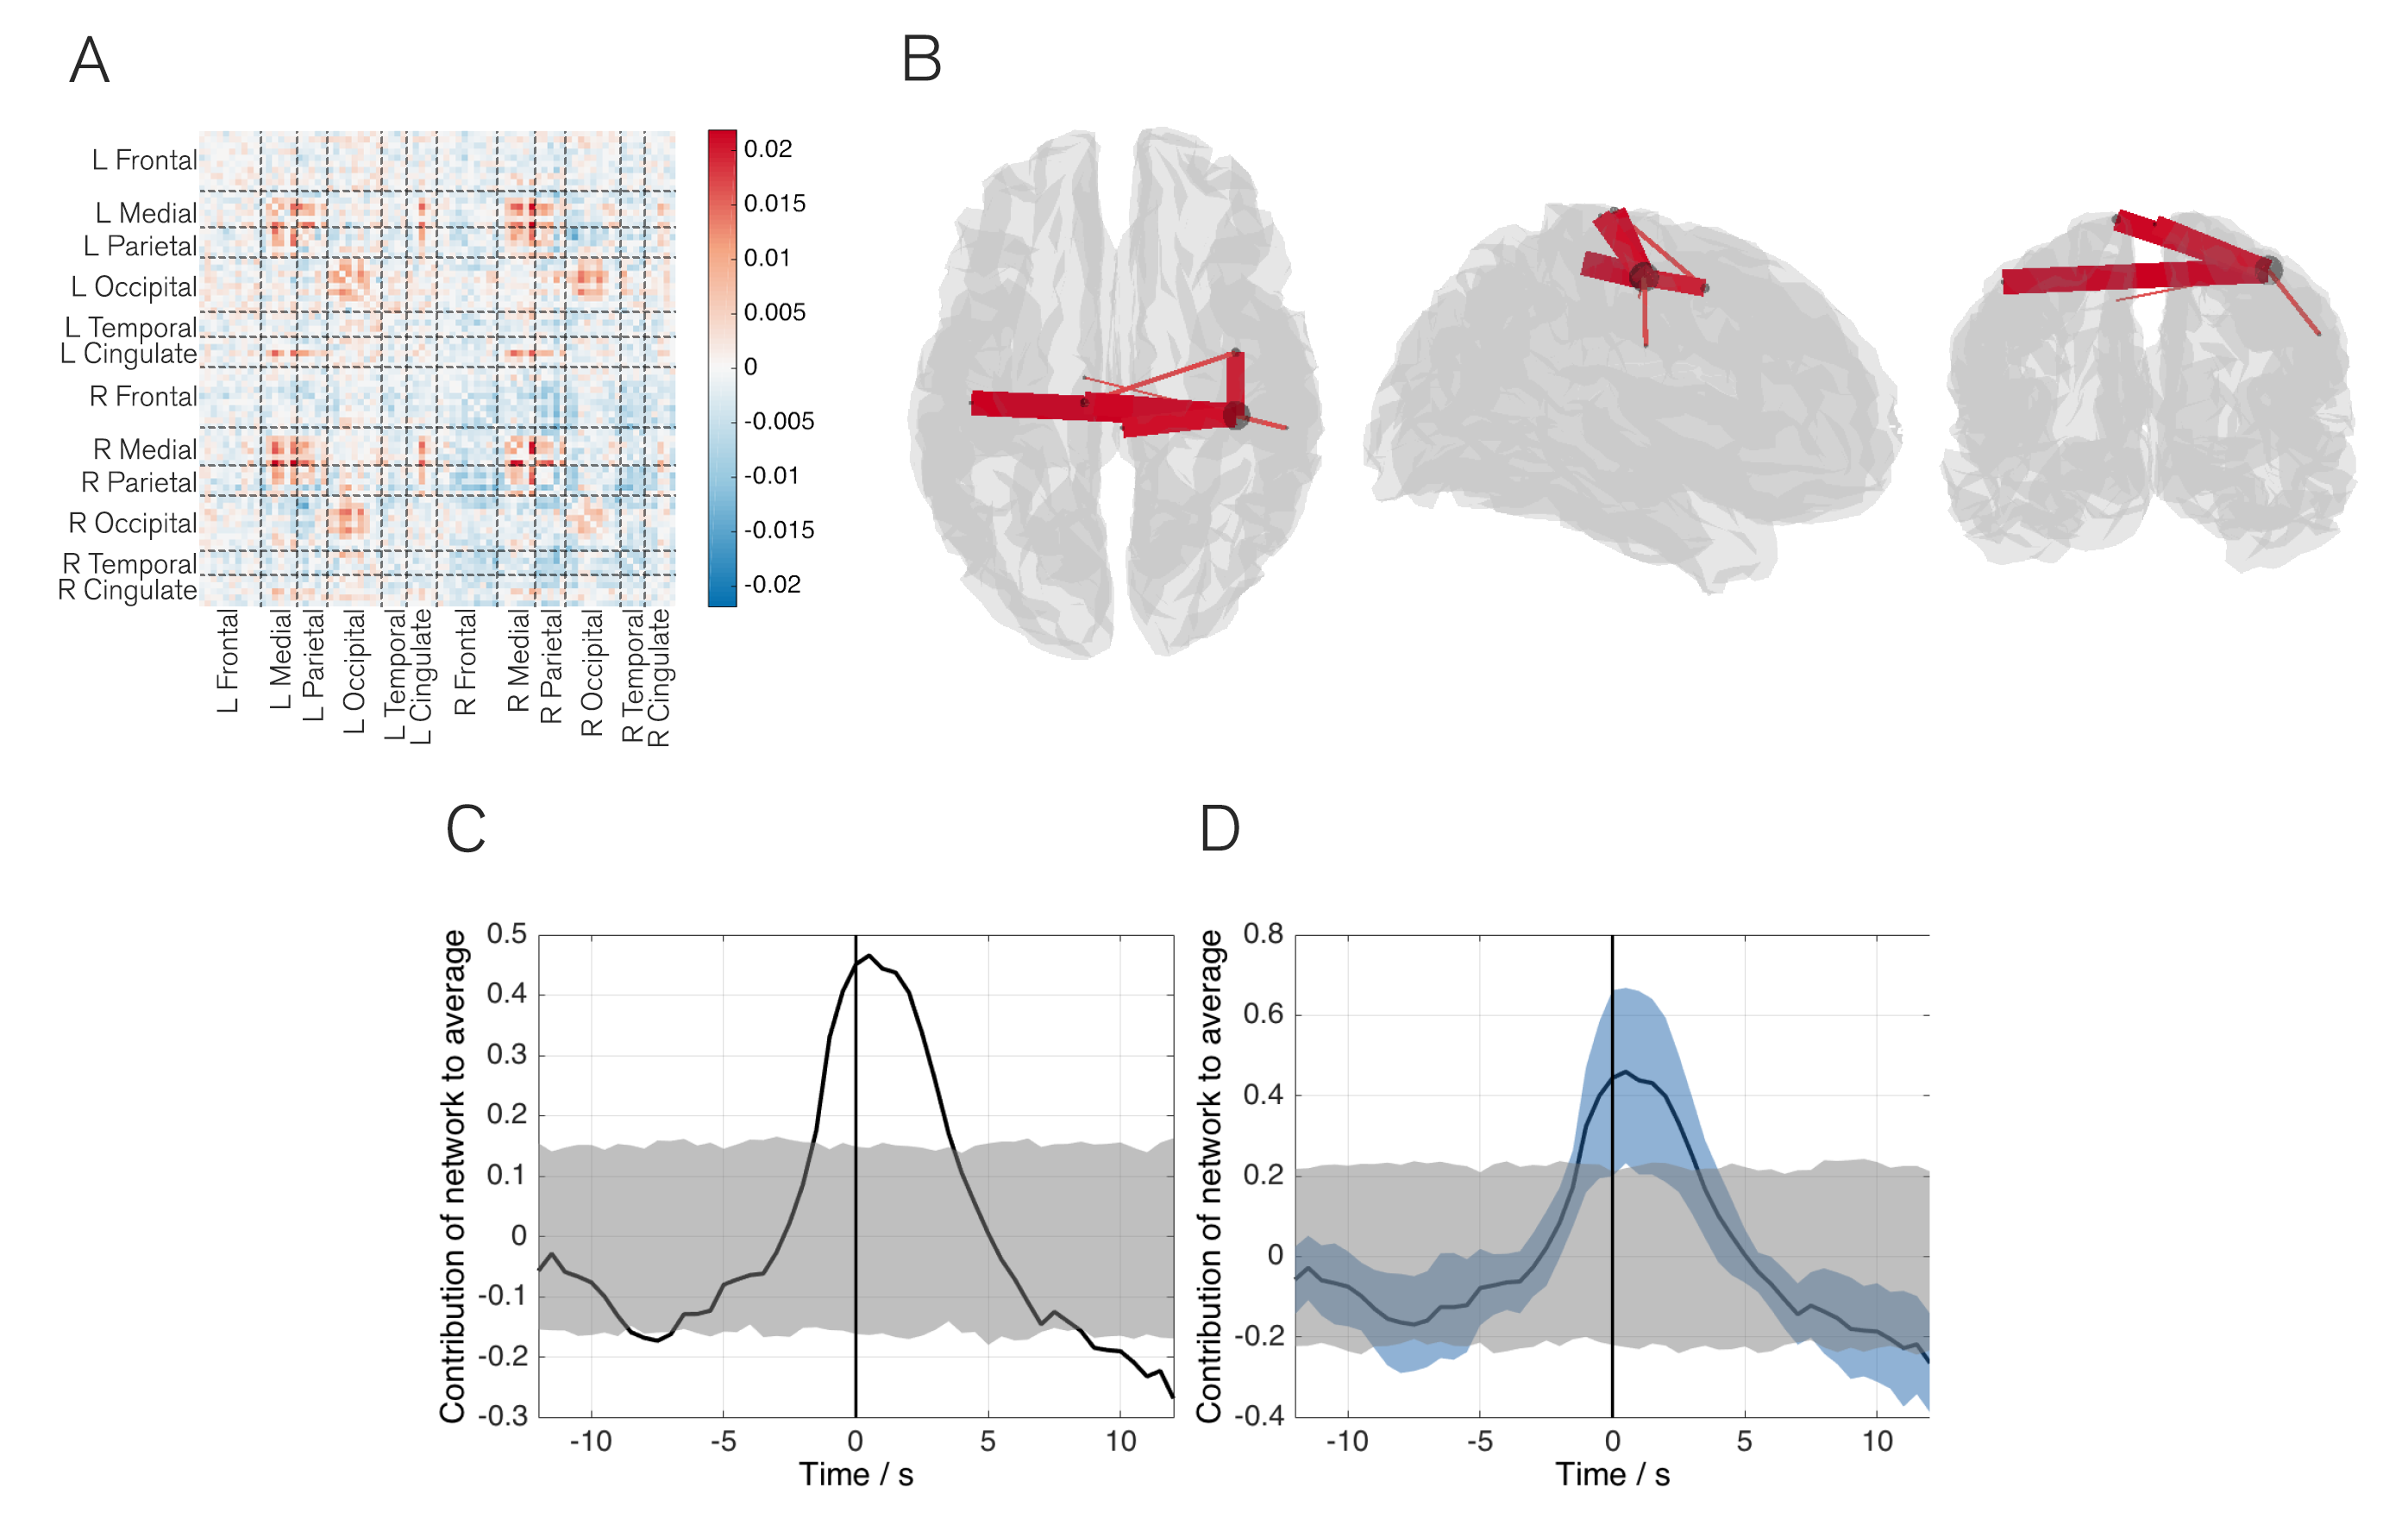
\includegraphics[width=\linewidth]{./images/chapter4/figure_2.png}\caption{Locations of simulated dipoles in the brain are shown by the blue overlay. The green overlay shows the volume covered by the seed and test voxel clusters.}\label{fig_4_2}
\end{figure}

Having simulated MEG data, the beamformer and CCA techniques were applied as described in Section \ref{sec_cca_theory} and summarised in Figure \ref{fig_4_3}. Beamformer projected timecourses were reconstructed on an 8mm grid within regions of interest covering the bilateral sensorimotor cortices. Those regions of interest are shown by the green overlay in Figure \ref{fig_4_2} and contained all six simulated sources. The seed cluster (containing 327 voxels) covered approximately the left motor strip and the test cluster (containing 274 voxels) covered approximately the right motor strip. Sliding window CCA was applied to source projected data in the beta band only, with a window width ($\delta$) of 30 s. The window was allowed to shift in time by $\delta t = 2$ s, giving a total of 230 overlapping windows. The dimensionality (\textit{d}) of the signals following eigenvalue decomposition of the windowed envelope matrices (i.e. the number of columns in $\mathbf{W}_{Xo}$ and $\mathbf{W}_{Yo}$) was set to 3.

\begin{figure}
	\includegraphics[width=\linewidth]{./images/chapter4/figure_3.png}\caption{Flowchart summarising the windowed CCA data analysis pipeline.}\label{fig_4_3}
\end{figure}

\clearpage
In order to test the statistical significance of the canonical correlation coefficients computed, multivariate phase randomisation, as describe by Equation \ref{eqn_4_24}, was employed. For each window, 1000 realisations of the randomised phase matrix ($\xi(f)$) were employed in order to generate surrogate matrices $\tilde{\mathbf{W}}_{X}$ and $\tilde{\mathbf{W}}_{Y}$. The CCA technique was then applied to these surrogate matrices in exactly the same way as that used for the real $\mathbf{W}_{X}$ and $\mathbf{W}_{Y}$. In this way a null distribution of correlation coefficients was generated independently for each time window. The upper 5th percentile was then computed with Bonferroni correction for multiple comparisons across independent time windows (each window was 30 s from a total of 490 s and hence a Bonferroni correction of 490/30 was applied). This was then used as a dynamic statistical threshold. This simulation was repeated with and without signal leakage correction.

In order to test further the validity of statistical testing via phase randomisation, a second simulation was undertaken. Here, the amount by which the window was allowed to shift in time ($\delta t$) was increased to 30 s, meaning that 15 non-overlapping (independent) time windows were employed. The number of iterations of the phase randomisation was reduced to 1, meaning that a single simulation produced 15 ‘real’ (i.e. based on simulated data) canonical correlation coefficients and 15 surrogate canonical correlation coefficients (based on phase randomised data). This whole processes was repeated 100 times, with the mean and the maximum canonical correlation coefficient, for both real and surrogate data, recorded on each iteration. Once again, this simulation was repeated with and without signal leakage correction. \clearpage

\subsubsection{Results}
Figure \ref{fig_4_4}A shows a spatial map, highlighting the effect of leakage correction on each voxel in the test cluster. The coloured overlay shows the magnitude of the mean square difference between the uncorrected \textbf{Y} and corrected $\mathbf{Y}_c$ test matrices, plotted across all voxels within the cluster. It is interesting to note that the effects of leakage vary spatially, with the largest effects observed in voxels closest to the seed cluster, as would be expected. Figures \ref{fig_4_4}B and \ref{fig_4_4}C show the timecourse of windowed canonical correlation (blue) for data with (\ref{fig_4_4}C) and without (\ref{fig_4_4}B) correction for signal leakage. The dynamic statistical threshold (\textit{p}\textsubscript{corrected}=0.05), generated by phase randomisation, is shown in red for both cases. Recall that this is a null simulation, with no expected coupling between sources and so the canonical correlation coefficients in the simulated data should remain below the statistical threshold. This is clearly the case for the leakage corrected data, but it is not the case for data without leakage correction where (spurious) significant coupling between voxels in the seed and test clusters is induced exclusively as a result of leakage. Figures \ref{fig_4_4}D and \ref{fig_4_4}E show histograms of canonical correlation coefficients; histograms in the upper panel were derived using phase randomised (null) data and histograms in the lower panel were derived directly from simulated data. Note that the upper panels in Figures \ref{fig_4_4}D and \ref{fig_4_4}E appear identical as the process of phase randomisation implicitly removes any leakage. Again the effect of leakage correction is obvious, with no observable difference between histograms in the case where correction is applied. Finally, Figures \ref{fig_4_4}F and \ref{fig_4_4}G show results of 100 iterations of the null simulation, with and without leakage correction respectively. Bar charts on the left hand side show the mean canonical correlation across 15 non-overlapping windows whereas bar charts on the right hand side show the maximum canonical correlation across windows. Results are shown for the simulated data and for the null distribution; error bars show standard deviation across the 100 iterations. Note that without correction, statistical testing via phase randomisation is clearly invalid, whereas following leakage correction, our simulation shows that a null distribution generated via phase randomisation represents an appropriate (if slightly conservative) statistical test.

\begin{figure}
	\includegraphics[width=\linewidth]{./images/chapter4/figure_4.png}\caption{Null simulations and the effect of leakage correction. A) Spatial map showing the mean effect of leakage correction on signals at each voxel. The colour overlay represents the mean square difference between the uncorrected \textbf{Y} and corrected $\mathbf{Y}_c$ matrices, averaged across all time and plotted across voxels; notice that the largest effects of signal leakage are distal to the sources, which are marked by the blue dots. B) and C) show timecourse of canonical correlation for simulated data (blue) and the \textit{p}\textsubscript{corrected}=0.05 dynamic statistical threshold (red). The case without leakage correction is shown in B and with leakage correction is shown in C. D) and E) show histograms of canonical correlation coefficients. The upper plots show null distributions derived using phase randomisation. The lower plots show distributions from simulated data. Note that without leakage correction (D) the mean canonical correlation computed using the simulated data is higher than the null distribution; since no temporal correlation has been simulated in this case, this is an example of spurious correlation. Note also that with leakage correction (E), the canonical correlation for the simulated corrected data is very similar to the null distribution, highlighting the fact that leakage correction eliminates the spurious correlations shown in (B). F) and G) show mean and maximum canonical correlation coefficients across 200 iterations of the null simulation (error bars show standard deviation). Note again the difference between leakage corrected (G) and uncorrected (F) data.}\label{fig_4_4}
\end{figure}

\subsection{Proof of Principle Simulation}
\subsubsection{Method}
The purpose of the second simulation was to test the beamforming and windowed CCA approach in the case where genuine coupling between dipole timecourses was simulated. Again six spatially separate sources were simulated at the same locations as those employed above (see Figure \ref{fig_4_2}). As previously, all six dipoles were orientated tangential to the radial orientation, with amplitude 3 nAm. Source timecourses were again generated as phase randomised versions of genuine (MEG measured) electrophysiological signals (490 s in duration), which were estimated from the motor cortex of a single individual during a resting state experiment. These were frequency filtered into the 13-30 Hz band. Temporal correlation between two sources was simulated within specific time windows, via multiplication by a modulatory function. To illustrate this mathematically, consider the case of two sources, labelled \textit{a} and \textit{b}. To impose coupling, we employ the following formulae:

\begin{align}
s_{a_{correlated}}(t_1 < \tau <t_2) &= s_{a_{uncorrelated}}(t_1 < \tau <t_2)M_{ab}(\tau) \label{eqn_4_25}\\
s_{b_{correlated}}(t_1 < \tau <t_2) &= s_{b_{uncorrelated}}(t_1 < \tau <t_2)M_{ab}(\tau) \label{eqn_4_26}
\end{align} Here, $s_{a_{uncorrelated}}$ and $s_{b_{uncorrelated}}$ represent the simulated neural signals for sources \textit{a} and \textit{b} respectively, in the absence of coupling. The window $(t_1 < \tau <t_2)$ designates the timing of the transient coupling between \textit{a} and \textit{b}. $M_{ab}(\tau)$ is a modulatory function which simulates temporal correlation and $s_{a_{correlated}}$ and $s_{b_{correlated}}$ represent the transiently coupled timecourses. $M_{ab}(\tau)$ was derived from a real MEG recording, and comprised genuine 70s segments of a beta band amplitude envelope, extracted via beamforming from the motor cortex of a single subject in the resting state  (data from \cite{Brookes2011a}). There were 6 simulated sources (labelled 1-6 in Figure \ref{fig_4_2}); coupling between sources 5 and 2 was simulated in the time window 50 s<\textit{t}<120 s; coupling between sources 3 and 4 was simulated in the time window 200 s<\textit{t}<270 s; coupling between sources 1 and 6 was simulated in the time window 350 s<\textit{t}<420 s. This generated three coupled source pairs defined by three independent modulatory functions $M_{52}(\tau)$,  $M_{43}(\tau)$ and $M_{61}(\tau)$. This methodology induces a transient (partial) temporal correlation between the amplitude envelopes of the source pairs, within the time windows specified. 

Following dipole timecourse generation, the simulation of MEG data was equivalent to that described in Section \ref{subaec_sim_method}. Timecourses were projected to the MEG sensors using a dipole forward solution and noise data added based on the empty room recording, generating a simulated dataset with SNR of 1.6. CCA was applied as described in section Figure \ref{fig_4_3}, with leakage correction.

\subsubsection{Results}
Figure \ref{fig_4_5} shows results of the proof of principle simulation. Figure \ref{fig_4_5}A represents the ground truth: that is, the temporal evolution of coupling between the simulated timecourses. The upper panel shows correlation between sources 5 and 2, the centre panel correlation between sources 3 and 4, and the lower panel correlation between sources 1 and 6. Note that the technique described by Equations \ref{eqn_4_25} and \ref{eqn_4_26} only induces a partial correlation between source pairs, with the magnitude of that correlation reaching an average of approximately 0.45 (Pearson correlation coefficient) within the windows of transient coupling. Figure \ref{fig_4_5}B shows the estimated canonical correlation as a function of time. The centre timecourse (blue line) shows the reconstructed temporal evolution of canonical correlation between the seed and test clusters. Note that since all six sources are captured within the clusters, correlation between all three coupled source pairs is captured in a single timecourse. The thin black line shows the dynamic statistical threshold (\textit{p}\textsubscript{corrected}=0.05) and the thick black line shows the mean of the null distribution (generated via phase randomisation) for each time window. Note that all three simulated interactions yield a significant result in the windowed CCA output. Interestingly, the dynamic statistical threshold also shows temporal structure with the mean of the null distribution, and the \textit{p}\textsubscript{corrected}=0.05 threshold, changing in time. These changes are driven by temporal structure in the autocorrelation of the envelope timecourses; this will be discussed further below. The spatial maps above and below the timecourse show individual images (derived from $\mathbf{I}_{WX}$ and $\mathbf{I}_{WY}$) depicting the spatial signature (canonical vectors) of correlation between the left and right clusters. These spatial maps are shown based on 30 s time windows centred at \textit{t} = 75 s, 100 s, 150 s, 225 s, 250 s, 300 s, 375 s and 400 s. Note that the change in spatial signature as a function of time is in agreement with the simulated connectivity. The blue dots show the locations of the simulated sources.

It should be noted that CCA is a multi-variate methodology and the output for each window is not a single value of canonical correlation, but rather multiple values, each reflecting a separate eigenmode of correlation (the number of modes is given by the minimum rank of $\mathbf{W}_{Xo}$, $\mathbf{W}_{Yo}$; in this case both have the same rank of \textit{d}). In the present simulation we used \textit{d}=3, thus there are three possible canonical modes of correlation. For completeness, Figure \ref{fig_4_6} shows the timecourse of the first eigenmode (blue line) alongside the timecourses of the second (red) and third (green) eigenmodes of correlation. As we artificially constructed a single spatial mapping between the voxels at any one time we would expect that the correlation between all source pairs is captured in the first eigenmode, with neither the second nor third eigenmodes showing significant deviation from zero.

\begin{figure}
	\includegraphics[width=\linewidth]{./images/chapter4/figure_5.png}\caption{Results of the proof of principle simulation. A) Shows the temporal evolution of simulated connectivity computed using timecourse data. The upper panel shows the timecourse of connectivity between sources 5 and 2; the centre panel shows the timecourse of connectivity between sources 3 and 4; the lower panel shows the timecourse of connectivity between sources 1 and 6. B) Connectivity reconstructed using CCA. The centre timecourse shows the reconstructed temporal evolution of connectivity between the seed and test clusters in the left and right motor strip respectively. Periods of significant temporal correlation are highlighted by the blue line passing outside the shaded region, which is bounded by a \textit{p}\textsubscript{corrected}=0.05 statistical threshold derived independently for each window but corrected for multiple time windows. The thick black line shows the mean canonical correlation for the null distribution, generated via phase randomisation. The spatial maps show individual images (i.e. $\mathbf{I}_{WX}$ and $\mathbf{I}_{WY}$) depicting the spatial signature (canonical vectors) of correlation between the left and right clusters. Note the change in spatial signature as a function of time is in agreement with the simulated connectivity. The blue dots show the locations of the simulated sources.}\label{fig_4_5}
\end{figure}

\begin{figure}
	\includegraphics[width=\linewidth]{./images/chapter4/figure_6.png}\caption{The timecourse of canonical correlation for all three eigenmodes. The blue line shows the first eigenmode which describes all of the simulated amplitude envelope correlation (note this is the same plot as that shown in Figure \ref{fig_4_5}B and is included here again for comparison). The green and red lines show the second and third eigenmodes respectively; note that in this case these higher modes exhibit no significant effect.}\label{fig_4_6}
\end{figure}
\clearpage

\section{Real MEG Data}\label{sec_cca_real}
\subsection{Methodology}
Following the application of windowed CCA in simulations, the same technique was applied to real resting state MEG data. A single subject was asked to lie in the scanner and 'think of nothing' for 600 s, acquisition procedures for this experiment are laid out in Section \ref{sec_data_acq}.

The acquired data post quality control were processed using the technique described in Section \ref{sec_cca_theory} and summarised in Figure \ref{fig_4_3}. Seed and test clusters were defined covering the left and right sensorimotor areas respectively; these regions are highlighted by the green overlay in Figure \ref{fig_4_7}A. Beamforming was applied in order to reconstruct timecourses of electrical activity on an 8 mm cubic grid spanning the seed and test clusters. The beamforming and CCA method (Figure \ref{fig_4_3}) was applied iteratively (treating each band independently) over multiple overlapping frequency bands (4-8 Hz, 6-10Hz, 8-13 Hz, 10-15 Hz and subsequent overlapping windows [10Hz bandwidth, 5Hz overlap] up to 105 Hz). For each band we used a fixed window width ($\delta$) of 40 s, a total of 280 windows, and a dimensionality (i.e. \textit{d}, the number of columns in $\mathbf{W}_{Xo}$ and  $\mathbf{W}_{Yo}$) of 3. The values of the canonical correlation coefficients, computed independently for each time window and frequency band, were used to construct a time-frequency (t-f) connectivity plot. This t-f connectivity plot was averaged, across all time windows, in order to calculate the average connectivity spectrum showing frequency bands that exhibit maximum envelope correlation.

Having computed canonical correlation across all frequencies, a single band of interest was identified for further analysis. MEG data were filtered in the 10-35 Hz band and again beamforming was applied to reconstruct timecourses on an 8 mm cubic grid spanning the seed and test clusters. CCA was applied, as described above, and images ($\mathbf{I}_{WX}$ and $\mathbf{I}_{WY}$) were computed within each time window. For each window, $\mathbf{I}_{WX}$ and $\mathbf{I}_{WY}$ (which represent the seed and test clusters respectively) were combined into a single image, thus generating a total of 280 separate spatial maps, each showing the weightings for voxels (canonical vectors) in the left and right sensorimotor region that describe optimal correlation between clusters. A timecourse of canonical correlation coefficients was also generated, and the significance of each coefficient computed using the phase randomisation approach, with correction for multiple comparisons across independent windows applied using the Bonferroni method. Although separate timecourses and image sets can be computed for each canonical mode, in this example only the dominant mode is considered. 

The set of 280 volumetric images (one per time window) show changes in the spatial signature of functional connectivity. However visualisation of this set of images is not trivial. In cases where a task has been employed, one might pick particular time windows that correspond to specific aspects of the task. In the present case however, since the MEG data represent subjects in a ‘resting’ state, any selection of time windows is somewhat arbitrary. A new set of problems therefore arise – how to identify the number of significantly different canonical vectors or spatial modes (see discussion). For simplicity we collapsed our 280 images into a smaller number of spatial patterns. To do this, first a covariance matrix was constructed, with dimension $280 \times 280$ whose \textit{ij}\textsuperscript{th} element contained the spatial covariance of image \textit{i} with image \textit{j}. This matrix was then decomposed into its constituent eigenvectors and eigenvalues. The eigenvectors were multiplied by the images in order to generate volumetric maps showing the spatial signature of each eigenmode; these maps are henceforth termed spatial modes and effectively represent orthogonal spatial patterns of connectivity observed within the 280 image set. The eigenvectors represent the weighting of each individual time window to a particular spatial mode, and can be thought of as a time series showing the contribution of each time point to that mode.

\subsection{Results}
Figure \ref{fig_4_7} shows the primary results of beamforming and windowed CCA applied to resting state MEG data. Figure \ref{fig_4_7}B shows the t-f connectivity plot, which facilitates visualisation of the temporal and spectral evolution of windowed band limited amplitude envelope correlation between voxel clusters in the left and right sensorimotor regions, in the resting state. Note the high degree of temporal and spectral non-uniformity: The value of canonical correlation exhibits a large variation in time, with high correlation ($\sim$0.6) in some windows and close to zero in other windows. Canonical correlation also exhibits a large degree of variation across frequency with the largest effects observed in the 8-35Hz frequency band. This is also evidenced by Figure \ref{fig_4_7}C, which shows the time average of canonical correlation plotted as a function of frequency. 

\begin{figure}[h!]
	\includegraphics[width=\linewidth]{./images/chapter4/figure_7.png}\caption{Resting state motor network connectivity. A) Green overlays show the anatomical locations of the seed and test clusters, in left and right sensorimotor regions respectively. B) Time frequency connectivity plot showing the temporal and spectral evolution of band limited amplitude correlation between voxel clusters in the left and right sensorimotor regions. C) Average connectivity spectrum, showing that the highest average motor network connectivity occurs in the alpha and beta bands.}\label{fig_4_7}
\end{figure}

The temporal and spatial variation of connectivity in the 10 – 35 Hz frequency band is shown in Figure \ref{fig_4_8}. The centre timecourse (blue line) shows the reconstructed temporal evolution of canonical correlation between the seed and test clusters in left and right sensorimotor cortices respectively. The thin black line shows the dynamic statistical threshold \textit{p}\textsubscript{corrected}=0.05) and the thick black line shows the mean of the null distribution (generated via phase randomisation) for each time window. Note that, in agreement with other results \citep{dePasquale2010,Baker2012} there is significant temporal variation in resting state correlation. As with the simulated data, the dynamic statistical threshold and mean canonical correlation calculated for the null distribution shows significant temporal structure. This temporal structure shows that a degree of temporal variability in metrics of functional connectivity can be generated purely via as a result of changes in the Fourier component that make up the source timecourses in a given window. This effect will be addressed further below. 

The spatial maps in Figure \ref{fig_4_8} show coronal and axial aspects of individual images depicting the spatial signature of correlation between clusters. These images are computed within 40 s time windows centred at t = 22 s, 80 s, 172 s, 226 s, 294 s, 460 s, 472 s and 562 s. The nature of resting state experiments means that these time points are selected somewhat arbitrarily (although all windows correspond to periods of significant temporal correlation). It is interesting to note that, in addition to the temporal and spectral variability shown by Figures \ref{fig_4_7} and \ref{fig_4_8}, a degree of spatial inhomogeneity in the network maps exists across separate time windows; and this will be addressed further in the discussion. 

Finally, Figure \ref{fig_4_9} shows the separate spatial modes of covariation computed using eigenvalue decomposition of a matrix of spatial covariance. (NB – spatial modes shown are distinct from the eigenmodes of CCA). The maps in Figure \ref{fig_4_9}A and \ref{fig_4_9}B show the first two spatial modes for a single subject. Note that two separate and distinct spatial patterns are observed. The first shows a symmetric spatial pattern involving bilateral primary sensorimotor cortices, approximately covering the hand area. This pattern has been commonly observed in previous studies. The second spatial mode, whilst again exhibiting symmetry across hemispheres, appears to show effects in inferior slices, possibly involving the secondary somatosensory region. Timecourses showing the contribution of each time window to the first and second spatial modes are shown in \ref{fig_4_9}C and \ref{fig_4_9}D respectively. For comparison, Figure \ref{fig_4_9}E shows a time average of all 280 images. 

\begin{figure}
	\includegraphics[width=\linewidth]{./images/chapter4/figure_8.png}\caption{Spatial patterns of connectivity in the 10–35 Hz frequency band. The centre (blue) timecourse shows the reconstructed temporal evolution of connectivity between the seed and test clusters in the left and right motor strip respectively. Periods of significant temporal correlation are highlighted by the blue line passing outside the shaded region, which is bounded by a \textit{p}\textsubscript{corrected}=0.05 statistical threshold derived independently for each window (and corrected for multiple windows). The thick black line shows the mean canonical correlation for the null distribution, generated via phase randomisation. The spatial maps show coronal and axial aspects of the individual images (i.e. $\mathbf{I}_{WX}$ and $\mathbf{I}_{WY}$) depicting the spatial signature of correlation between the left and right clusters within 30 s time windows centred at selected time points t = 22 s, 80 s, 172 s, 226 s, 294 s, 460 s, 472 s and 562 s. Note that there is a degree of spatial inhomogeneity over time.}\label{fig_4_8}
\end{figure}

\begin{figure}
	\includegraphics[width=\linewidth]{./images/chapter4/figure_9.png}\caption{Spatial modes of correlation. A) and B) show the first and second spatial modes of correlation respectively; the timecourses showing the contribution of each time window to the first and second spatial modes are shown in C and D. E) shows the simple time average of all 280 images.}\label{fig_4_9}
\end{figure}

\clearpage
\section{Discussion}\label{sec_cca_discuss}
The next generation of tools to compute functional connectivity in neuroimaging data must account for temporal non-stationarity, spatial inhomogeneities, and spectral structure. Here, we have presented a means to achieve this via application of beamforming and windowed CCA to MEG data. We have shown it possible to generate time-frequency connectivity plots showing the temporal and spectral evolution of coupling between brain regions. Moreover, CCA over voxels provides a means to assess spatial inhomogeneity within those short time-frequency windows. We have demonstrated the feasibility of this technique in simulation, and using real MEG data.

In this chapter, we extended a previous idea for leakage suppression based on removal of linear (zero-phase-lag) interactions (Chapter \ref{sec_signal_corr}; \cite{Brookes2012b,Hipp2012}) between beamformer projected source time series in the seed and test clusters. Source leakage between voxels in MEG source space is necessarily zero-phase-lag and removal of this component has been demonstrated by previous papers \citep{Brookes2012b,Hipp2012} as an effective means to suppress spurious interactions. Here we extended the regression idea from the univariate case presented previously in Chapter \ref{chapter_fc_and_leakage}, to a multivariate case. This extension facilitates removal of linear interaction between all voxels (and all linear mixtures of voxels) in the seed and test clusters. As expected, the magnitude of the effect of this correction differs across voxels within the clusters; this was shown in Figure \ref{fig_4_4}A, with the largest degree of correction in voxels located in close proximity to the seed cluster. Empirical evidence for the success of this method was given in Figures \ref{fig_4_4}B – \ref{fig_4_4}G. Without correction, canonical correlation coefficients between the seed and test cluster were much higher in the simulation than for a phase randomised case. Recall that phase randomisation not only destroys genuine correlation (i.e. functional connectivity) but also destroys spurious correlation caused by leakage. This means that prior to correction, a significant difference in canonical correlation between simulated and phase randomised data would be expected and driven entirely by leakage – this was observed in Figures \ref{fig_4_4}B, D and F. Following correction however, this difference would be expected to be eliminated, and this was indeed evidenced by Figures \ref{fig_4_4}C, E and G. The empirical evidence presented therefore adds weight to previous studies \citep{Brookes2012b,Hipp2012} showing that regression based leakage correction is effective.

Despite this success, further work is required to characterise fully this technique and potential problems still remain.  Firstly, leakage suppression comes at the expense of the loss of any genuine zero phase lag interactions between the seed and test clusters; this may be problematic in cases where, for example, a single (e.g. thalamic) source drives two cortical sources with zero-phase-lag. Secondly, the assumptions of constant leakage across all time is not necessarily valid. As shown in Chapter \ref{sec_signal_leakage}, the magnitude of source leakage is dependent on the variance of the source being reconstructed. It therefore follows that if the variance of a source between windows varies, then the leakage profile shall also. This is not unfeasable as we know that the source variance can vary greatly; for example, in a motor activity the event related attentuation on beta-band power and the following resynchronisation would with (if windows were short enough) show a marked change in variance between them. This is investigated further in Chapter \ref{chap_kmeans}, where we attempt to assess functional connectivity on shorter temporal scales. In the context of this investigation, it could be speculated that the variance of a source across a long temporal window (such as the 40 s in this chapter) may not show a distinct change in source variance between windows -- especially given that the data is resting state.

The windowed CCA approach allows assessment of the temporal evolution of functional connectivity between the seed and test clusters. Furthermore, application within multiple frequency bands enables effective measurement of the spectral signature of temporal correlation. Multiple previous studies \citep{Chang2010,dePasquale2010,Brookes2011a,Baker2012,dePasquale2012} have shown that functional connectivity is dynamic and that temporal correlation between spatially separate brain areas exhibits large changes in time; this observation has been made using both fMRI and MEG. The results presented in Figures \ref{fig_4_7} and \ref{fig_4_8} are in agreement with this, showing large dynamic changes in canonical correlation between the left and right motor clusters. In addition our results show strong frequency dependence with the highest values of temporal correlation observed in the alpha and beta frequency band; this again is in agreement with previous literature \citep{Mantini2007,Brookes2011a,Hipp2012}. One of the problems with measurement of temporal correlation in short windows is that of SNR. MEG data exhibit inherently low SNR, and the data captured within the small time-frequency windows used here are unaveraged, making accurate measurement of temporal coupling challenging. CCA, applied across voxels, is helpful in this context since is allows a principled way to generate a weighted average of signals across multiple voxels in source space. Averaging voxel timecourses in this way enables an effective increase in the SNR of the data, and hence a more accurate means to assess the time-frequency evolution of connectivity. 

Statistical thresholding to define time-frequency windows exhibiting significant temporal correlation is non-trivial. As described in Section \ref{phase_randomisation}, changes in the temporal profile of correlation can be generated simply as a result of changes in the temporal autocorrelation of the envelope time series across multiple time windows. Such temporal structure in the envelope timecourse for the seed and test regions will yield changes in correlation; such changes are trivial, and driven not by a genuine change in functional coupling between regions, but by changes in the Fourier components that make up the signal. In this chapter, we apply a previously described technique \citep{Prichard1994} to correct for such trivial changes in canonical correlation by employing a dynamic statistical test based on multivariate phase randomisation. By building a null distribution based on Equation \ref{eqn_4_24}, we ensure that the canonical correlation coefficients defining that null are constructed using surrogate windowed envelope timecourses with the same autocorrelation function as the real data. This means that any changes in correlation driven purely by changes in signal characteristics are accounted for. It is interesting to note that, in real MEG data, this approach yields a dynamic statistical threshold that exhibits marked changes in time. Future work using MEG (or fMRI) to measure dynamic changes in functional connectivity should bear this issue in mind, and employ phase randomisation or alternative techniques to compute dynamic thresholds.

As with all neuroimaging methodologies, windowed CCA requires selection of a parameter set upon which the algorithm is based. The key parameters are 1); the voxel cluster size, 2) the number of eigenmodes (\textit{d}) retained within each window and 3) the time frequency window size. Judicious selection of regions of interest is key to the CCA technique. If regions are made too small, one loses spatial degrees of freedom and ultimately the CCA technique collapses to univariate correlation. Alternatively, if regions are made to large, one may dilute the effects of interest in specific brain areas, by incorporating other regions which contribute orthogonal signals. Selection of regions of interest, for the present study, was based upon the sensorimotor network previously defined by fMRI \citep{Smith2012}, however it is equally possible to select regions based on cortical parcellation. Ultimately, region selection depends on the precise scientific question to be addressed. Selecting the number of retained eigenmodes, \textit{d}, is linked directly to both the volume encompassed by the selected regions (larger regions require increased \textit{d}) and the spatial resolution of the MEG inverse projection within those regions (higher spatial resolution means more independent signals within a cortical volume, necessitating larger \textit{d}). This means that, again, selection of \textit{d} is specific to the particular study being undertaken; this said an objective means to select \textit{d} can be derived as the percentage of data variance explained by the eigenmodes retained. Finally, judicious selection of a time frequency window involves a trade-off between temporal/spectral resolution and accuracy. The smaller the time frequency window, the less accurate the estimation of temporal correlation. The window size is also related to the number of selected eigenmodes (\textit{d}) and, as a rule of thumb, one requires more than 4\textit{d} independent temporal observations within the window for the multivariate test to be reliable. This imposes a fundamental limit on temporal resolution of any sliding window technique. However in this chapter we have not reached the limit as to how short the window can possibly be; the 40 s width can be made considerably shorter (indeed, it can be seen in \ref{fig_4_5}, the due to the low temporal resolution that such a wide window possesses, the onset and offset of interactions in the simulation are deemed insignificant by our null hypothesis, suggesting the temporal resolution can be improved). Reducing the window width will prove particularly useful for investigating task-based modulations in functional connectivity, which we investigate this in Chapter \ref{chap_kmeans}. 

A powerful and complementary alternative to sliding windows, which has particular application in resting state MEG measurements, is to deploy techniques such as Hidden Markov Models (HMMs), which have been shown to detect short-lived re-occurring states in resting state MEG data, characterised by repeating patterns of covariance over channels \citep{Woolrich2013,Baker2014}. This multivariate approach has, so far, been used to perform temporally adaptive MEG source reconstruction and could be readily extended for use with CCA, to detect repeating patters of connectivity produced from the outputs of CCA, or even to infer connectivity at the source level between clusters of interest directly with HMMs, bypassing CCA altogether. It should also be noted that, in addition to these fundamental parameters, windowed CCA as described is critically dependent of source localisation, in this case using beamforming. Parameter selection and optimised application of beamforming is covered extensively in previous literature (Chapter \ref{chapter_meg_source}; \citealp{Brookes2008}) and will not be reproduced here. However, we do note that windowed CCA may, in principle, by applied in conjunction with any inverse projection technique, with the caveat that different inverse projection algorithms exhibit different signal leakage characteristics and the interaction between inverse projection and leakage correction should be characterised prior to direct application.

Assessment of spatial non-stationarity in functional connectivity is important if we are to generate a means to measure the spatial signature of ‘sub-networks’ within previously characterised large scale distributed networks. The CCA approach, as presented, allows a means to measure changes in the spatial signature of connectivity throughout the experiment. The utility of the method was demonstrated by application to the resting state data in Figures \ref{fig_4_8} and \ref{fig_4_9}. These results cannot be over interpreted since, although the spatial patterns elucidated have been shown to be consistent over one individual, they may not readily extend to a large group. This said, it is clear from Figure \ref{fig_4_8} that a degree of spatial inhomogeneity is apparent within the motor network, with spatially distinct ‘sub-networks’ exhibiting significant canonical correlation within temporally separated windows. This result was extended further in Figure \ref{fig_4_9}, with the inclusion of volumetric maps depicting two separate spatial modes of correlation. The first spatial mode resembles strongly a well-known sensorimotor network, which is often observed in both bilateral and unilateral motor paradigms. This comprises bilateral and symmetric regions covering (approximately) the hand areas of left and right sensorimotor cortex. The second spatial mode incorporates bilateral and symmetric cortical regions observed in inferior slices. The inherent smoothness of MEG images necessarily makes unambiguous spatial interpretation of these images challenging, but nevertheless this secondary spatial mode is physiologically plausible, and may incorporate the bilateral secondary somatosensory region. Similar spatial patterns were found in a second individual during a resting state MEG acquisition. Methods to derive robust and regularly occurring spatial patterns of connectivity offer a means to extend the CCA technique from single subject application (as presented) to group study. Techniques such as eigenvalue decomposition (as used here) or alternatively k-means clustering (\citealp{MacQueen1967,Allen2014,Liu2013} which will be introduced in Chapter \ref{chap_kmeans}), should allow elucidation of consistent spatial patterns across multiple subjects. Alternatively, it is conceivable that concatenating spatially normalised volumetric images across many subjects may generate large multi-subject datasets amenable to processing with techniques such as spatial ICA, which again may elucidate robust and regularly occurring spatial patterns of functional sub-networks within (for example) the sensorimotor system. Although it has not been demonstrated in this chapter whether the results presented can be seen across multiple subjects, they do present an immediate example of the utility of the windowed CCA approach. In Chapter \ref{chap_kmeans} we implement CCA across multiple group studies and provide principled methods to identify spatial and temporal modes of connectivity in MEG.  

\section{Conclusion}
The results presented in this chapter show that a combination of beamforming, multivariate leakage correction, and windowed CCA is a simple and flexible approach to measure the 5-dimensional evolution of functional connectivity, assessed by temporal correlation of band limited oscillatory amplitude. The utility of this approach has been shown in simulation, and in real resting state MEG data. We have also shown that there are distinct spatial modes of connectivity within previously established functional networks. The existence of these is exciting as they may be the constituent connections within a 'static' functional network which rapidly form and dissolve based on the current mental state. Their origins and functional meanings haven't yet been elucidated, but in Chapter \ref{chap_kmeans}, we take the methods introduced to measure multidimensional dynamic connectivity and use them to investigate how functional connectivity within the sensorimotor network (and its constituent subnetworks) evolves within multiple studies.  